        %auto-ignore
\begin{figure}[h]
    \centering
    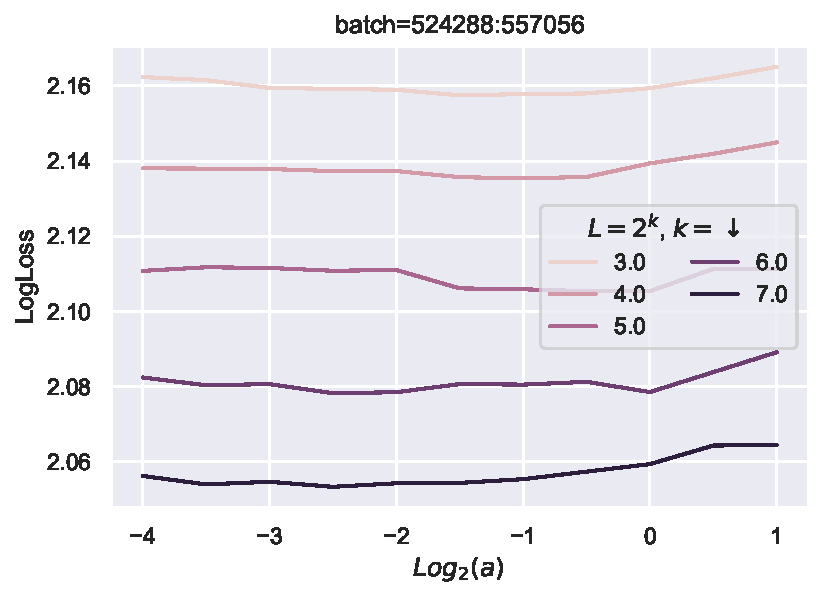
\includegraphics[width=0.45\linewidth]{fig/megatron_bm_insensitive_524288.pdf}
    \caption{Modern transformers are insensitive to block multiplier $a$.}
    \label{fig:megatron_bm_insensitive}
\end{figure}

\begin{figure}[h]
    \centering
    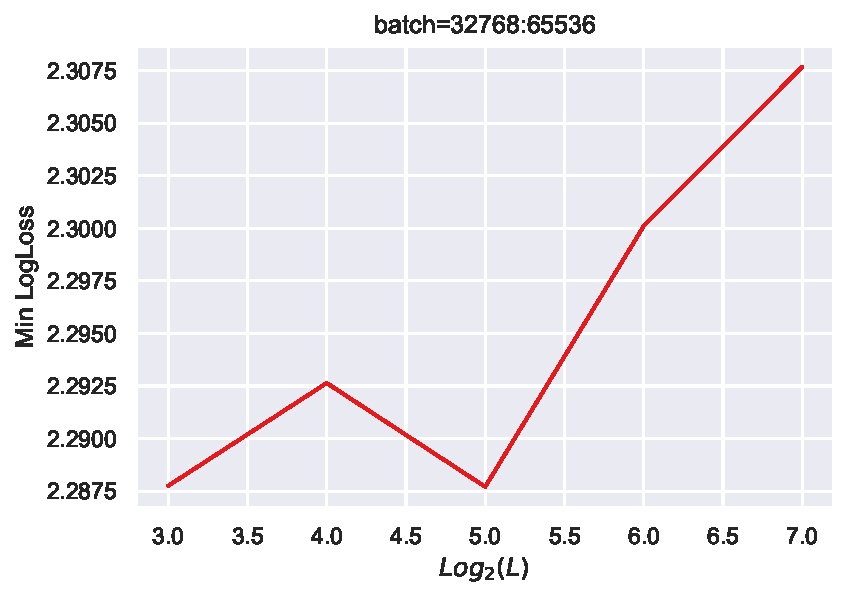
\includegraphics[width=0.4\linewidth]{fig/megatron_minimal_loss_32768.pdf}
    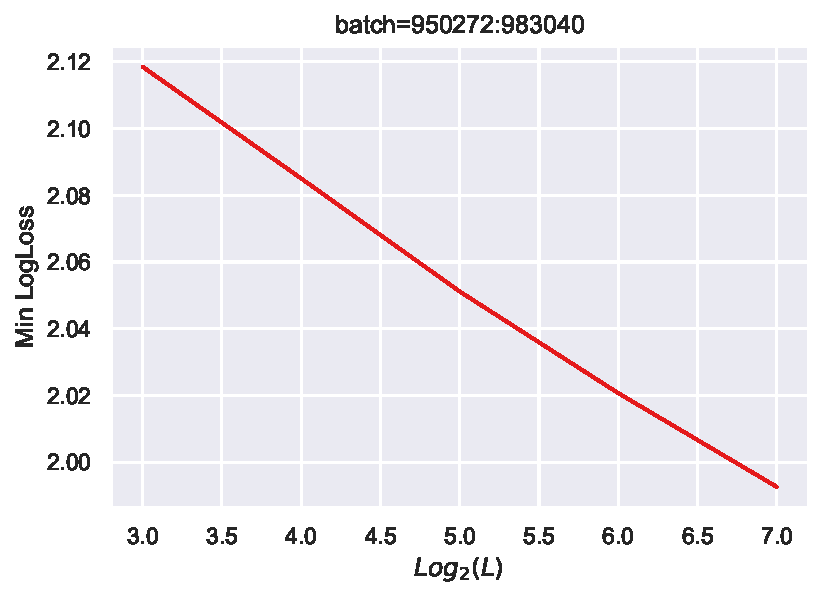
\includegraphics[width=0.4\linewidth]{fig/megatron_minimal_loss_950272.pdf}
    \caption{In (Megatron) Transformer trained on Common Crawl, deeper does worse initially (Left) but eventually does better (Right).}
    \label{fig:megatron-deeper-worse}
\end{figure}

\begin{figure}[h]
    \centering
    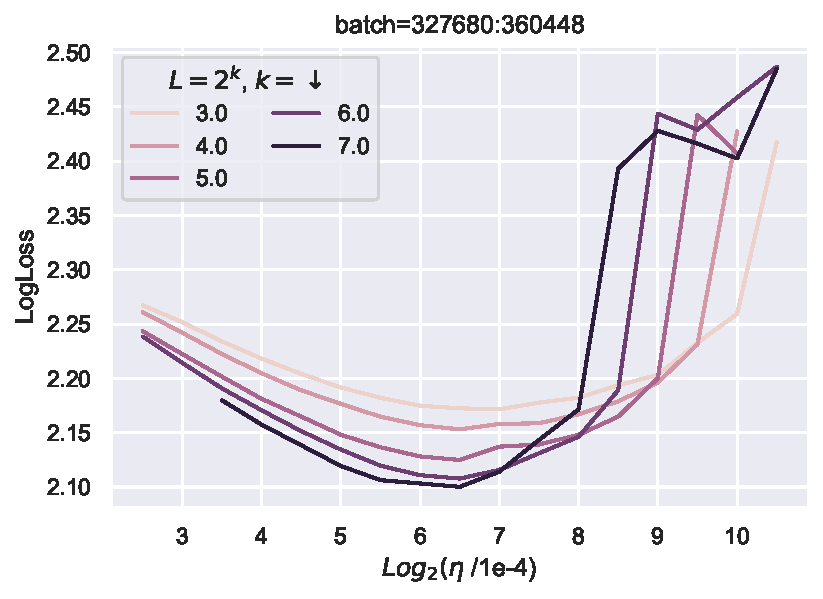
\includegraphics[width=0.4\linewidth]{fig/megatron_1scaling_327680.pdf}
    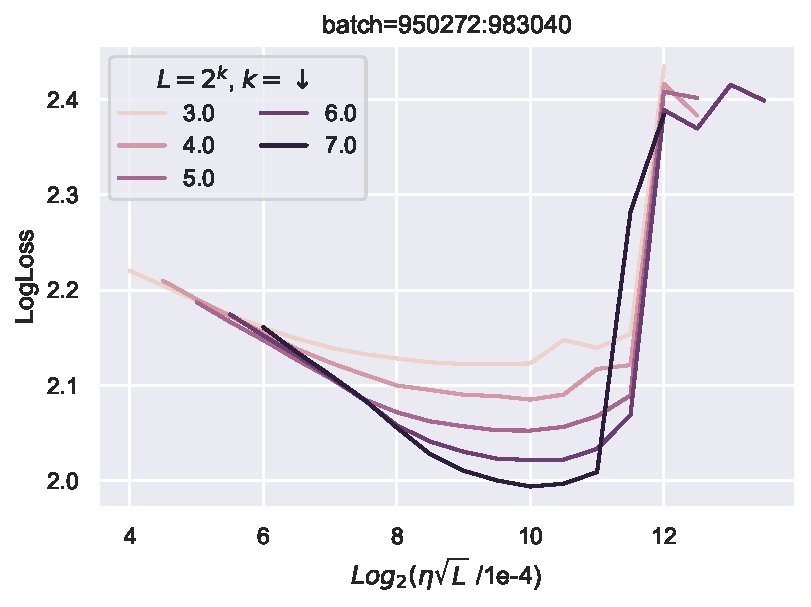
\includegraphics[width=0.4\linewidth]{fig/megatron_sqrt_scaling950272.pdf}
    \caption{In the middle of (Megatron) transformer training, optimal learning rate is approximately invariant (Left), while at the end of training, it approximately scales like $1/\sqrt{L}$. However, the $1/\sqrt{L}$ scaling transfers the maximum viable learning rate better in either case. }
    \label{fig:megatron-scaling-shifts}
\end{figure}

\section{What Happens in a Transformer?}

Because transformers have block depth 2, as discussed in \cref{sec:bd2}, we have plenty of reasons to suspect that no parametrization of (learning rate, block multiplier) will be able to robustly transfer hyperparameters across depth for transformers.

Here we do a large scale experiment using Megatron trained on Common Crawl and catalogue our observations.\footnote{3900 steps, warmup 500 steps (cosine decay to lr 1e-6), sequence length 4096, batch size 256. In total approximately 4B tokens.}
In summary, in our particular setup (which should be close to most large language model pretraining), we see that the $1/\sqrt L$ scaling seems to transfer hyperparameters at the end of training (\cref{{fig:megatron-scaling-shifts}}(Right)). However, we also see that 1) deeper does worse in initial training (\cref{{fig:megatron-deeper-worse}}(Left)), and 2) optimal hyperparameters scale like $\Theta(1)$ in the middle of training (\cref{fig:megatron-scaling-shifts}(Left)).
Combined with the theoretical insights of \cref{sec:bd2}, this leads us to conclude that while the $1/\sqrt L$ scaling can potentially be practically useful in transformer training, it is likely to be brittle to architectural  and algorithmic changes, or even simple things like training time.

In fact, we observe that transformers are insensitive to the block multiplier $a$ (\cref{fig:megatron_bm_insensitive}), so that the only relevant hyperparameter is really just learning rate. Thus, empirically measuring the scaling trend of the optimal learning rate, as done in modern large scale pretraining, can be a practically more robust way to transfer hyperparameters.

Here $L$ is the number of transformer layers, each of which consists of an attention layer and an MLP layer (each of which has depth 2).

